\documentclass[xcolor=table,bigger,unknownkeysallowed]{beamer}
\usetheme{SimplePlus}
\usepackage[utf8]{inputenc}
\usepackage[T1]{fontenc}
\usepackage[english]{babel}
\usepackage{fixltx2e}
\usepackage{graphicx}
\usepackage{epsfig}
\usepackage{longtable}
\usepackage{float}
\usepackage{wrapfig}
\usepackage{soul}
\usepackage{textcomp}
\usepackage{marvosym}
\usepackage{wasysym}
\usepackage{latexsym}
\usepackage{amssymb}
\usepackage{tabu}
\usepackage{tabularx}
\usepackage{booktabs}
\usepackage[margin=15pt,font={small,sf,it},labelfont=bf]{caption} 
\usepackage{hyperref}
\tolerance=1000
\providecommand{\alert}[1]{\textbf{#1}}
\usepackage{etoolbox}
\newcommand{\icon}[1]{\includegraphics[height=20pt,width=20pt]{#1}}
\usepackage{pgfplots}
\usepackage{tabu}
\usepackage{subcaption}
\usepackage{multirow}
\usepackage{pdfpages}

\usepackage{tikz}
\usetikzlibrary{matrix,positioning,fit,fadings}
\def\drowsyColor{green!80!black}       

\title{Out of Hypervisor (OoH): Efficient Dirty Page Tracking In Userspace Using Hardware Virtualization Features}
\author{\textit{Stella Bitchebe \& Alain Tchana, SC22, November 17$^{th}$ 2022}}
\date{~}
% More styles for bullets
\usepackage{pifont}
\usepackage{booktabs}
\usepackage[natbib=true, bibstyle=authoryear, citestyle=authoryear-comp]{biblatex}
\usepackage{beamerthemesplit}
\usetheme{progressbar}
\usecolortheme{progressbar}
%\institute{\vskip1ex Rennes - April, 29}
\definecolor{tableShade}{HTML}{787878}
\definecolor{tableShade2}{HTML}{606060}
\progressbaroptions{headline=none, frametitle=ckcompliant}
\newcommand{\myitem}{\item[\vspace{0.5ex}]}
\newcommand{\myemph}[1]{\textcolor{red}{\bf #1}}
\usepackage{lmodern}
\usepackage{ulem} 

\AtBeginSection[]
{
  \begin{frame}<beamer>%{Outline}
	\thispagestyle{empty}
    %\tableofcontents[sectionstyle=show/shaded,subsectionstyle=show/shaded/hide]
	\small \tableofcontents[currentsection,hideothersubsections]
	\addtocounter{framenumber}{-1}
  \end{frame}
}
% \AtBeginSubsection[]    %\frametitle{Outline for section \thesection}

% {
%   \begin{frame}<beamer>{Outline}
% 	\tableofcontents[currentsubsection]% Only one option does make sense here
%   \end{frame}
% }

% \subsection{State-of-the-art}
% \begin{frame}<beamer>
% 	\tableofcontents[sectionstyle=show/hide,subsectionstyle=show/shaded/hide]
% \end{frame}
\setbeamersize{text margin left=0em,text margin right=0em}

\usepackage{tikz,pgfplots}
\usetikzlibrary{pgfplots.groupplots}
\usepackage{pgfplotstable}
\usepgfplotslibrary{external} 
\usetikzlibrary{patterns}
\usepgfplotslibrary{fillbetween}
\usetikzlibrary{matrix,positioning,fit,fadings}
\tikzfading[name=energyPropFading,bottom color=transparent!100,top color=transparent!0]
\usepackage{color, colortbl}
\hypersetup{}

\definecolor{codegreen}{rgb}{0,0.6,0}
\definecolor{codegray}{rgb}{0.5,0.5,0.5}
\definecolor{codepurple}{rgb}{0.58,0,0.82}
\definecolor{backcolour}{rgb}{0.95,0.95,0.92}
\definecolor{americanrose}{rgb}{1.0, 0.01, 0.24}
\definecolor{airforceblue}{rgb}{0.0, 0.0, 1.0}

\newenvironment{variableblock}[3]{% 3 args
  \setbeamercolor{block body}{#2} %2nd arg
  \setbeamercolor{block title}{#3}
  \begin{block}{#1}}{\end{block}
}

\newenvironment{coloredtitleblock}[1]{% 
  \begin{block}{\textcolor{blue}{\bf #1}}}{\end{block}
}

\tikzfading[name=myfading, bottom color=transparent!100, top color=transparent!0]

% \logo: bottom right
%\logo{
\includegraphics[width=.15\linewidth]{images/logobottom.png}}

\begin{document}

\setbeamertemplate{headline}{\hfill
\includegraphics[width=.15\linewidth]{images/logobottom.png}\hspace{0.2cm}\vspace{-.8cm}}

%\setbeamertemplate{footline}{
\includegraphics[width=.15\linewidth]{images/logobottom.png}\hspace{-6cm}\vspace{2cm}}

\frame[plain]{
\includegraphics[page=1,width=\textwidth]{title.pdf}}
%\maketitle

%%%%%%%%%%%%%%%%%%%%%%%%%%%%%%%%%%%%%%%%%%%%%%%%%%%%%%%%%%%%%%%%%%%%%%%%%%%%%%%%%%%
%\section{Context: }
%%%%%%%%%%%%%%%%%%%%%%%%%%%%%%%%%%%%%%%%%%%%%%%%%%%%%%%%%%%%%%%%%%%%%%%%%%%%%%%%%%%
% \begin{frame}
% 	\frametitle{Why the Cloud?} 
% 	\begin{itemize}
% 		\item Attractive costs (e.g., \textit{Faas})
% 		\item Management tasks simplification (e.g., \textit{SaaS, IaaS})
% 		\item Efficiency of Cloud computing, including for HPC applications
% 		\item Several HPC FaaS platforms beeing developped (e.g., \textit{funcX}\footnote<.(1)->{Allows to execute millions of functions across thousands of nodes in the Cloud.})
% 	\end{itemize}
% \end{frame}
% -------------------------------
% \begin{frame}
% 	\frametitle{Virtualized Cloud Infrastructure} 	
% 	\begin{figure}
% 	\centering
% 	\fcolorbox{white}{white}{
% 		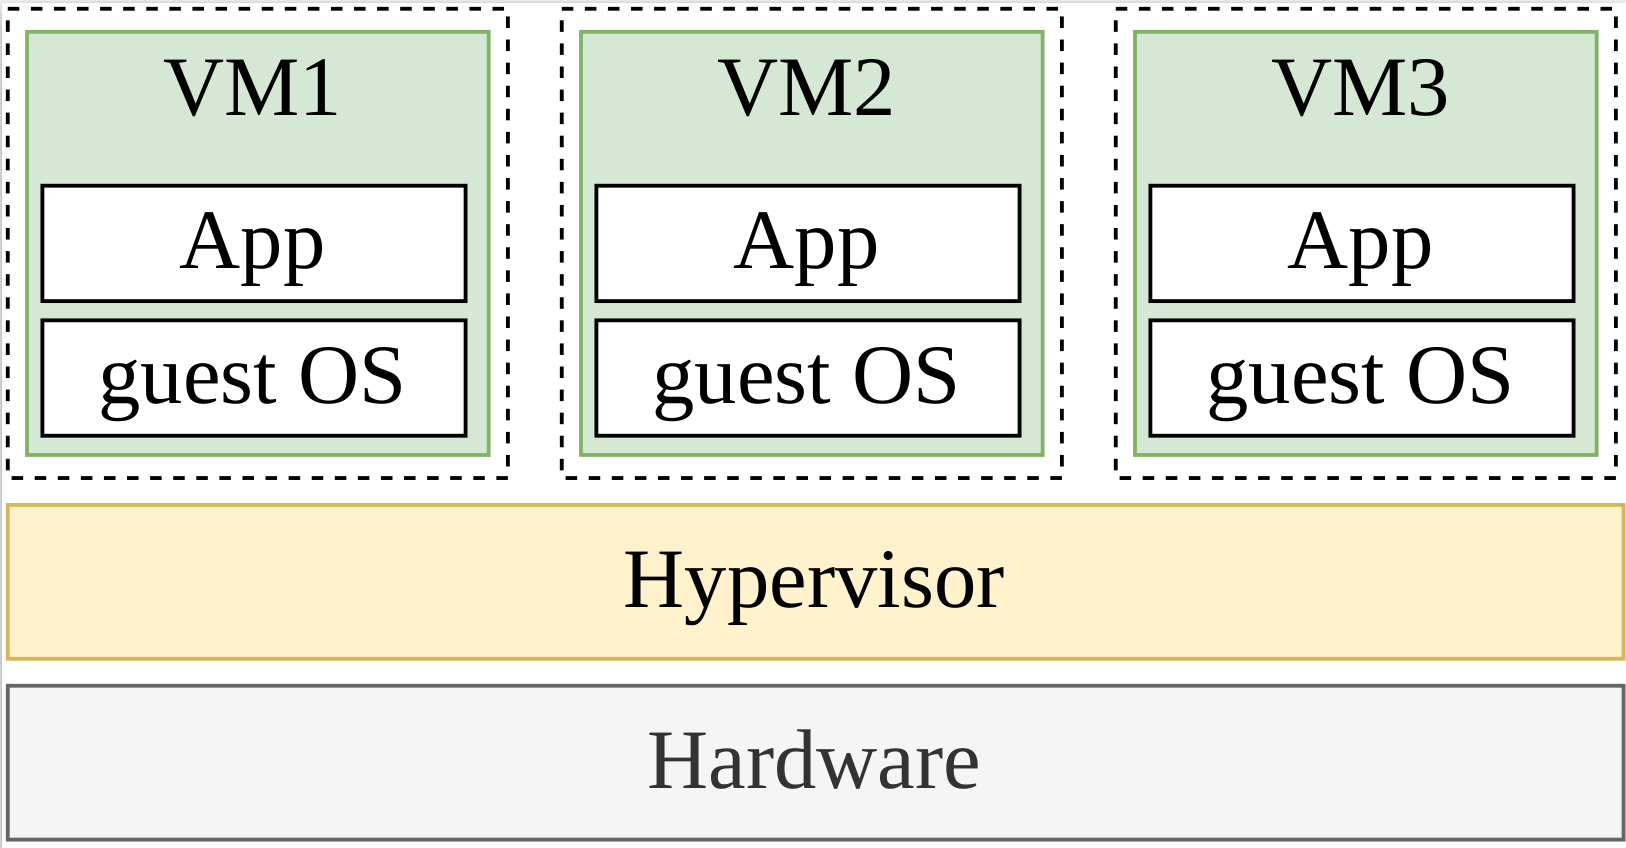
\includegraphics[width=.5\columnwidth]{fig/type1.png}
% 	}
% 	\end{figure}
% \end{frame}

%%%%%%%%%%%%%%%%%%%%%%%%%%%%%%%%%%%%%%%%%%%%%%%%%%%%%%%%%%%%%%%%%%%%%%%%%%%%%%%%%%%
\section{Virtualized Clouds: Dirty Page Tracking in Guest Userspace}
\subsection{Importance}
\subsection{State-of-the-art Techniques}
%%%%%%%%%%%%%%%%%%%%%%%%%%%%%%%%%%%%%%%%%%%%%%%%%%%%%%%%%%%%%%%%%%%%%%%%%%%%%%%%%%%
\begin{frame}
\frametitle{Virtualized Clouds: Dirty Page Tracking in Userspace} 
	\begin{block}{Purpose}
		\begin{itemize}
			\item WSS (working set size) estimation (\textit{for memory overcommitment})
			\item Live migration (\textit{for maintenance})
			\item Checkpointing (\textit{for recovery after failure})
			\item Garbage collection (\textit{for better memory management})
		\end{itemize}
	\end{block}	
		
	\pause

	\begin{block}{Nomenclature}
		\begin{itemize}
			\item Tracker: the monitoring thread (e.g., CRIU, Boehm GC)
			\item Tracked: the thread whose memory is monitored (any application)
		\end{itemize}
	\end{block}	
\end{frame}
%---------------------------------------------
% \begin{frame}
% \frametitle{Dirty Page Tracking in Userspace} 		
% \begin{block}{Overall Functioning}
% 	\begin{itemize}
% 		\item Tracker's activity can be organized in four phases: 
% 		\begin{itemize}
% 			\item the initialization of the tracking method
% 			\item the monitoring
% 			\item the collection of dirty page addresses
% 			\item the exploitation of the latter (e.g., for checkpointing)
% 		\end{itemize}
% 	\end{itemize}
% \end{block}	
% \end{frame}
%---------------------------------------------
\begin{frame}
\frametitle{Virtualized Clouds: Dirty Page Tracking in Userspace} 
	\begin{block}{Current approach}
		\begin{itemize}
			\item Page write protection
			\item Two main solutions
			\begin{itemize}
				\item Linux /proc interface
				\item Linux userfaultfd (ufd) interface
			\end{itemize}
		\end{itemize}
	\end{block}	
	\begin{figure}
	\centering
		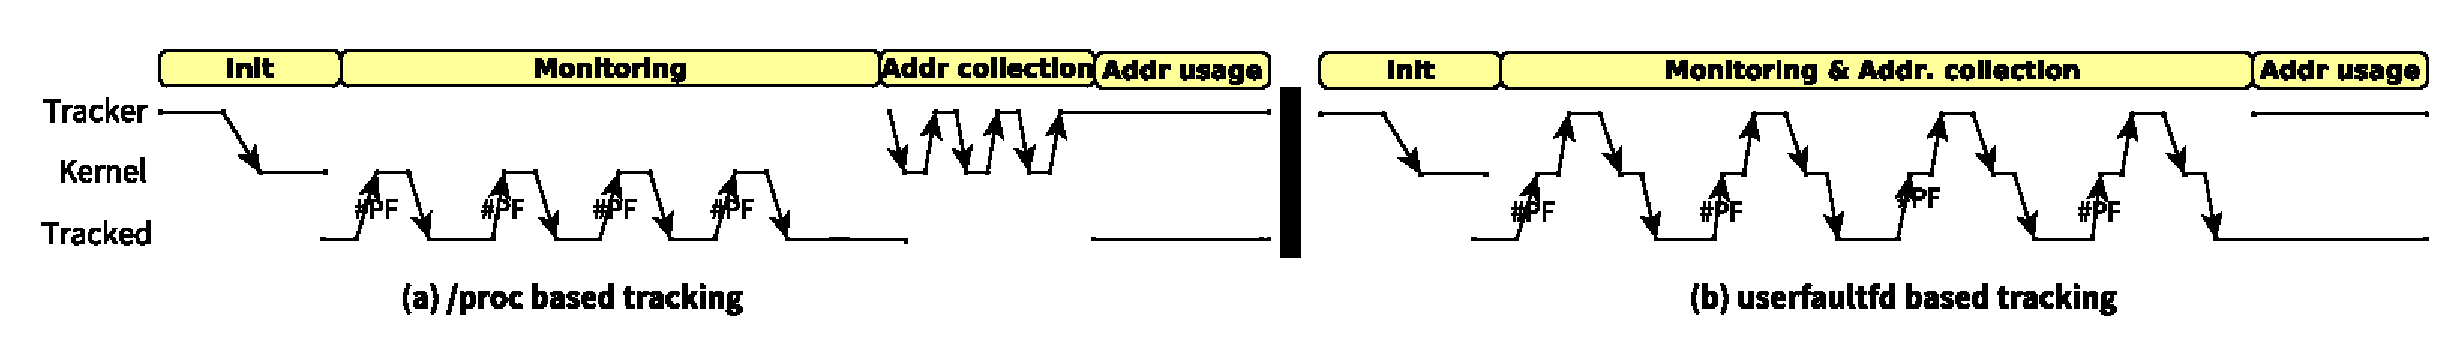
\includegraphics[width=1\columnwidth]{fig/solutions1}
	\end{figure}
\end{frame}

%%%%%%%%%%%%%%%%%%%%%%%%%%%%%%%%%%%%%%%%%%%%%%%%%%%%%%%%%%%%%%%%%%%%%%%%%%%%%%%%%%%
\section{Problem: Limits of Existing Solutions}
%%%%%%%%%%%%%%%%%%%%%%%%%%%%%%%%%%%%%%%%%%%%%%%%%%%%%%%%%%%%%%%%%%%%%%%%%%%%%%%%%%%
\begin{frame}
	\frametitle{Problem: Limits of Page Write Protextion} 
	%\begin{block}{Overhead}
	\emph{Overhead}\\
	\begin{itemize}
		\item ufd: Page fault (\#PF) handling and context switches
		\begin{itemize}
			\item \myemph{15.6$\times$} and \myemph{14.5$\times$} slowdown for 1GB on Tracked and Tracker respectively
		\end{itemize}
		\pause
		\item /proc: \#PF handling and page table (PT) walks
		\begin{itemize}
			\item \myemph{$\sim$2.234ms}: parse PT and flush TLB (in the kernel)
			\item \myemph{$\sim$594.187ms}: parse PT in userspace (/proc/PID/pagemap) for 1GB				
			\item \myemph{4.3$\times$} and \myemph{2.5$\times$} slowdown for 1GB on Tracked and Tracker respectively
		\end{itemize}					
	\end{itemize}
	%\end{block}				
\end{frame}                   

%%%%%%%%%%%%%%%%%%%%%%%%%%%%%%%%%%%%%%%%%%%%%%%%%%%%%%%%%%%%%%%%%%%%%%%%%%%%%%%%%%%   
\section{Solution: Hardware-Assisted Virtualization Out of Hypervisor (OoH)}
\subsection{Virtualization Technologies}
\subsection{Categorization of Virtualization Technologies}
\subsection{OoH Principle}
%%%%%%%%%%%%%%%%%%%%%%%%%%%%%%%%%%%%%%%%%%%%%%%%%%%%%%%%%%%%%%%%%%%%%%%%%%%%%%%%%%%
\begin{frame}
	\frametitle{Virtualization Technologies}
	\begin{itemize}
		\item Goal: reduce overheads of virtualization
		\item AMD-v (2006) and Intel VT (2005)
		\begin{itemize}
			\item CPU virtualization (e.g., VT-x)
			\item MMU virtualization (e.g., EPT)
			\item I/O virtualization (e.g., SRIOV)
		\end{itemize}
	\end{itemize}	
\end{frame}
% ----------------------------
\begin{frame}
	\frametitle{Intel VT Features Categorization}
	2 main groups:
	\begin{block}{\textcolor{blue}{\bf $G_1$: Multiplexing Features}}
		\begin{itemize}
			\item Extended Page Table (EPT)
			\item Single Root I/O Virtualization (SRIOV)
			\item Advanced Programmable Interrupt Controller virtualization (APICv)
		\end{itemize}
	\end{block}
	\pause
	\begin{block}{\textcolor{blue}{\bf $G_2$: Management Features}}
		\begin{itemize}
			\item Page Modification Logging (PML)
			\item Sub-Page write Permissions (SPP)
			\item Cache Allocation Technology (CAT)
		\end{itemize}		
	\end{block}
	\pause
	$G_2$'s features can be exploited in VMs
\end{frame}
% ----------------------------
\begin{frame}
	\frametitle{OoH Principle}
	\begin{itemize}
		\item \myemph{New research axis}
		\item Objective
		\begin{itemize}
			\item Make some hardware virtualization features usable within the guest OS
			\item From conception/design of features
		\end{itemize}
		\pause
		\item Methodology
		\begin{itemize}
			\item Kernel module and userspace library
			\item Hypercalls and event channels between hypervisor and guests
			\item Leverage existing extensions for direct passthrough
			\item Hardware changes (e.g., ISA extension)
		\end{itemize}		
	\end{itemize}
\end{frame}

%%%%%%%%%%%%%%%%%%%%%%%%%%%%%%%%%%%%%%%%%%%%%%%%%%%%%%%%%%%%%%%%%%%%%%%%%%%%%%%%%%%   
\section{OoH for PML}
\subsection{PML Functioning}
\subsection{Shadow PML (SPML)}
\subsection{Extended PML (EPML)}
\subsection{Security and Isolation}
%%%%%%%%%%%%%%%%%%%%%%%%%%%%%%%%%%%%%%%%%%%%%%%%%%%%%%%%%%%%%%%%%%%%%%%%%%%%%%%%%%%
\begin{frame}
\frametitle{PML Functioning} 
	Allows the hypervisor to track guest memory accesses\\
	\begin{figure}
		\centering
		%\fcolorbox{white}{white}{					
		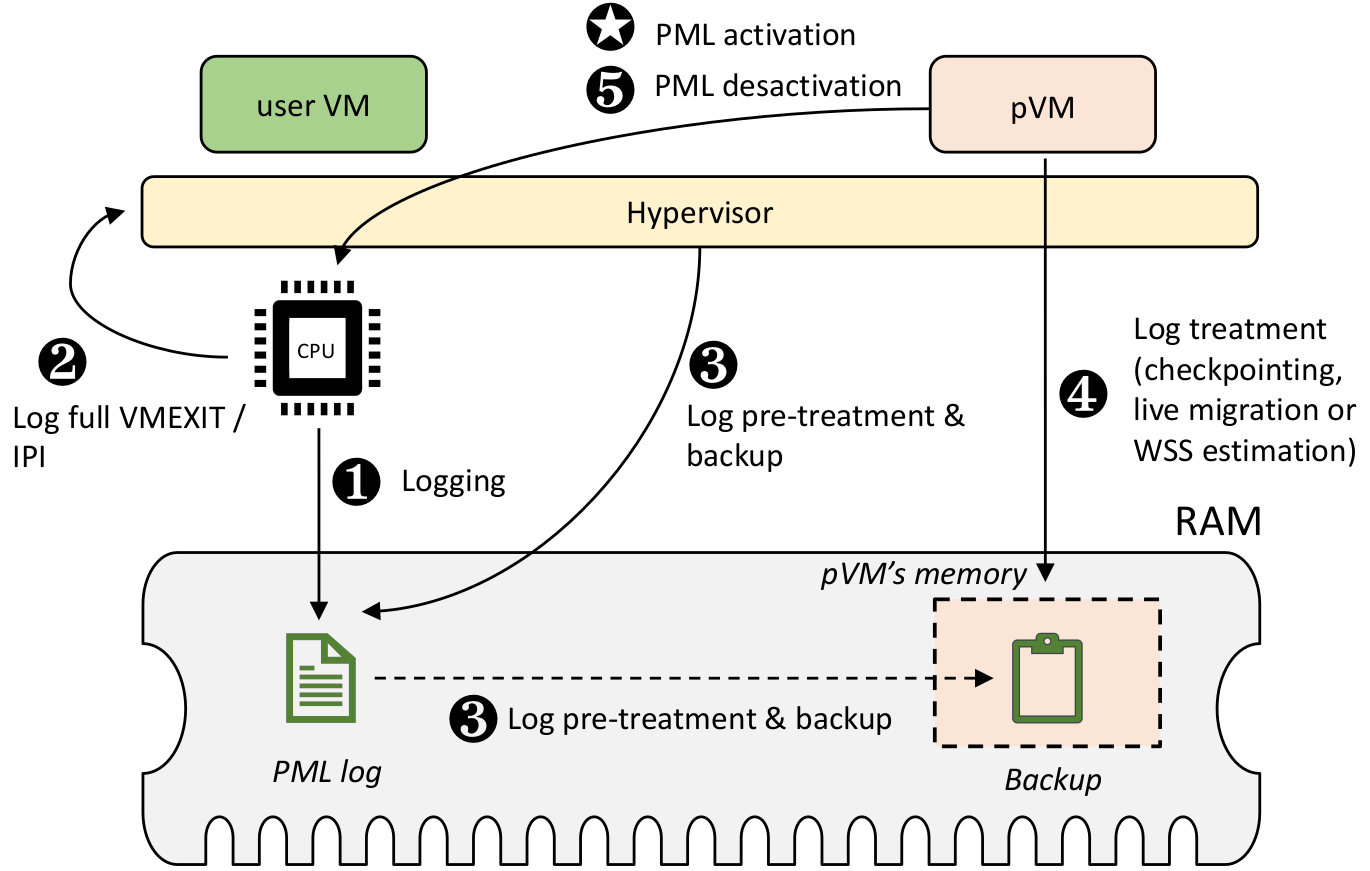
\includegraphics[width=.55\columnwidth]{fig/pml_actual}
		%}
	\end{figure}
	
	\begin{block}{Intel PML in the OoH Context}
		\begin{itemize}
			\item To accelerate CRIU checkpointing and Boehm garbage collection
		\end{itemize}
	\end{block}				
\end{frame}
%---------------------------------
\begin{frame}
\frametitle{PML-based Dirty Page Tracking in Userspace} 
	\begin{figure}
	\centering
		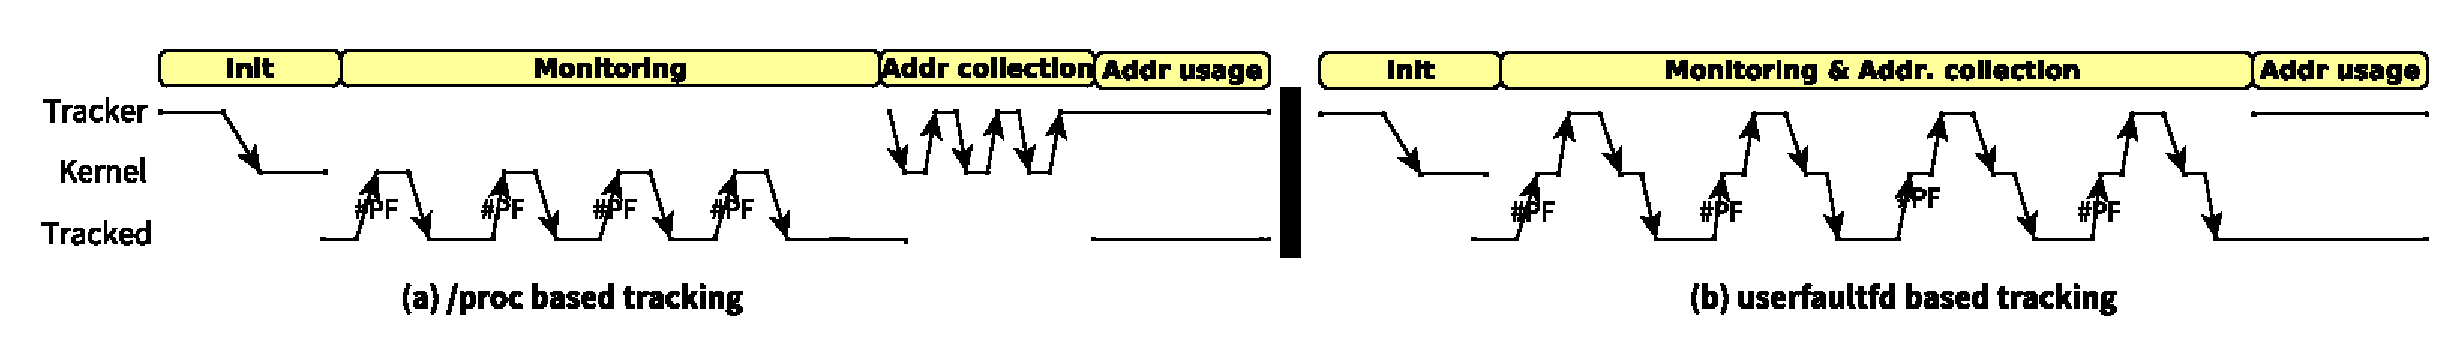
\includegraphics[width=1\columnwidth]{fig/solutions1}
	\end{figure}
~\\			
~\\
	\begin{figure}
	\centering
		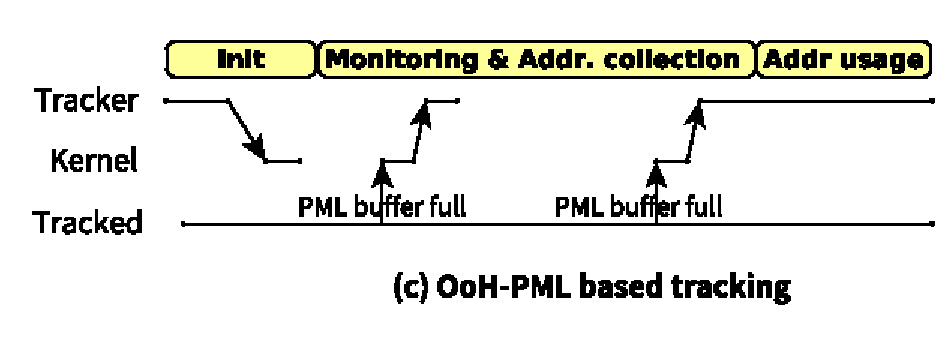
\includegraphics[width=.6\columnwidth]{fig/solutions2}				
	\end{figure}							
\end{frame}          
%---------------------------------
\begin{frame}
	\frametitle{OoH for PML}	
	% \begin{overprint}

	% 	\onslide<1>		
	\begin{block}{Challenges}
		\begin{itemize}
			\item ($C_1$) PML can only be managed by the hypervisor
			\item ($C_2$) PML works at coarse-grained, that is it concerns the entire VM
			\item ($C_3$) PML only logs GPAs
		\end{itemize}
	\end{block} 

	% \onslide<2>	
	% \begin{figure}
	% 	\centering
	% 		\begin{subfigure}{.48\linewidth}
	% 			\centering			
	% 			\begin{block}{Challenges}
	% 				\begin{itemize}
	% 					\item ($C_1$) PML can only be managed by the hypervisor
	% 					\item ($C_2$) PML works at coarse-grained, that is it concerns the entire VM
	% 					\item ($C_3$) PML only logs GPAs
	% 				\end{itemize}	
	% 			\end{block} 			
	% 		\end{subfigure}
	% 		\begin{subfigure}{.48\linewidth}
	% 			\centering
	% 			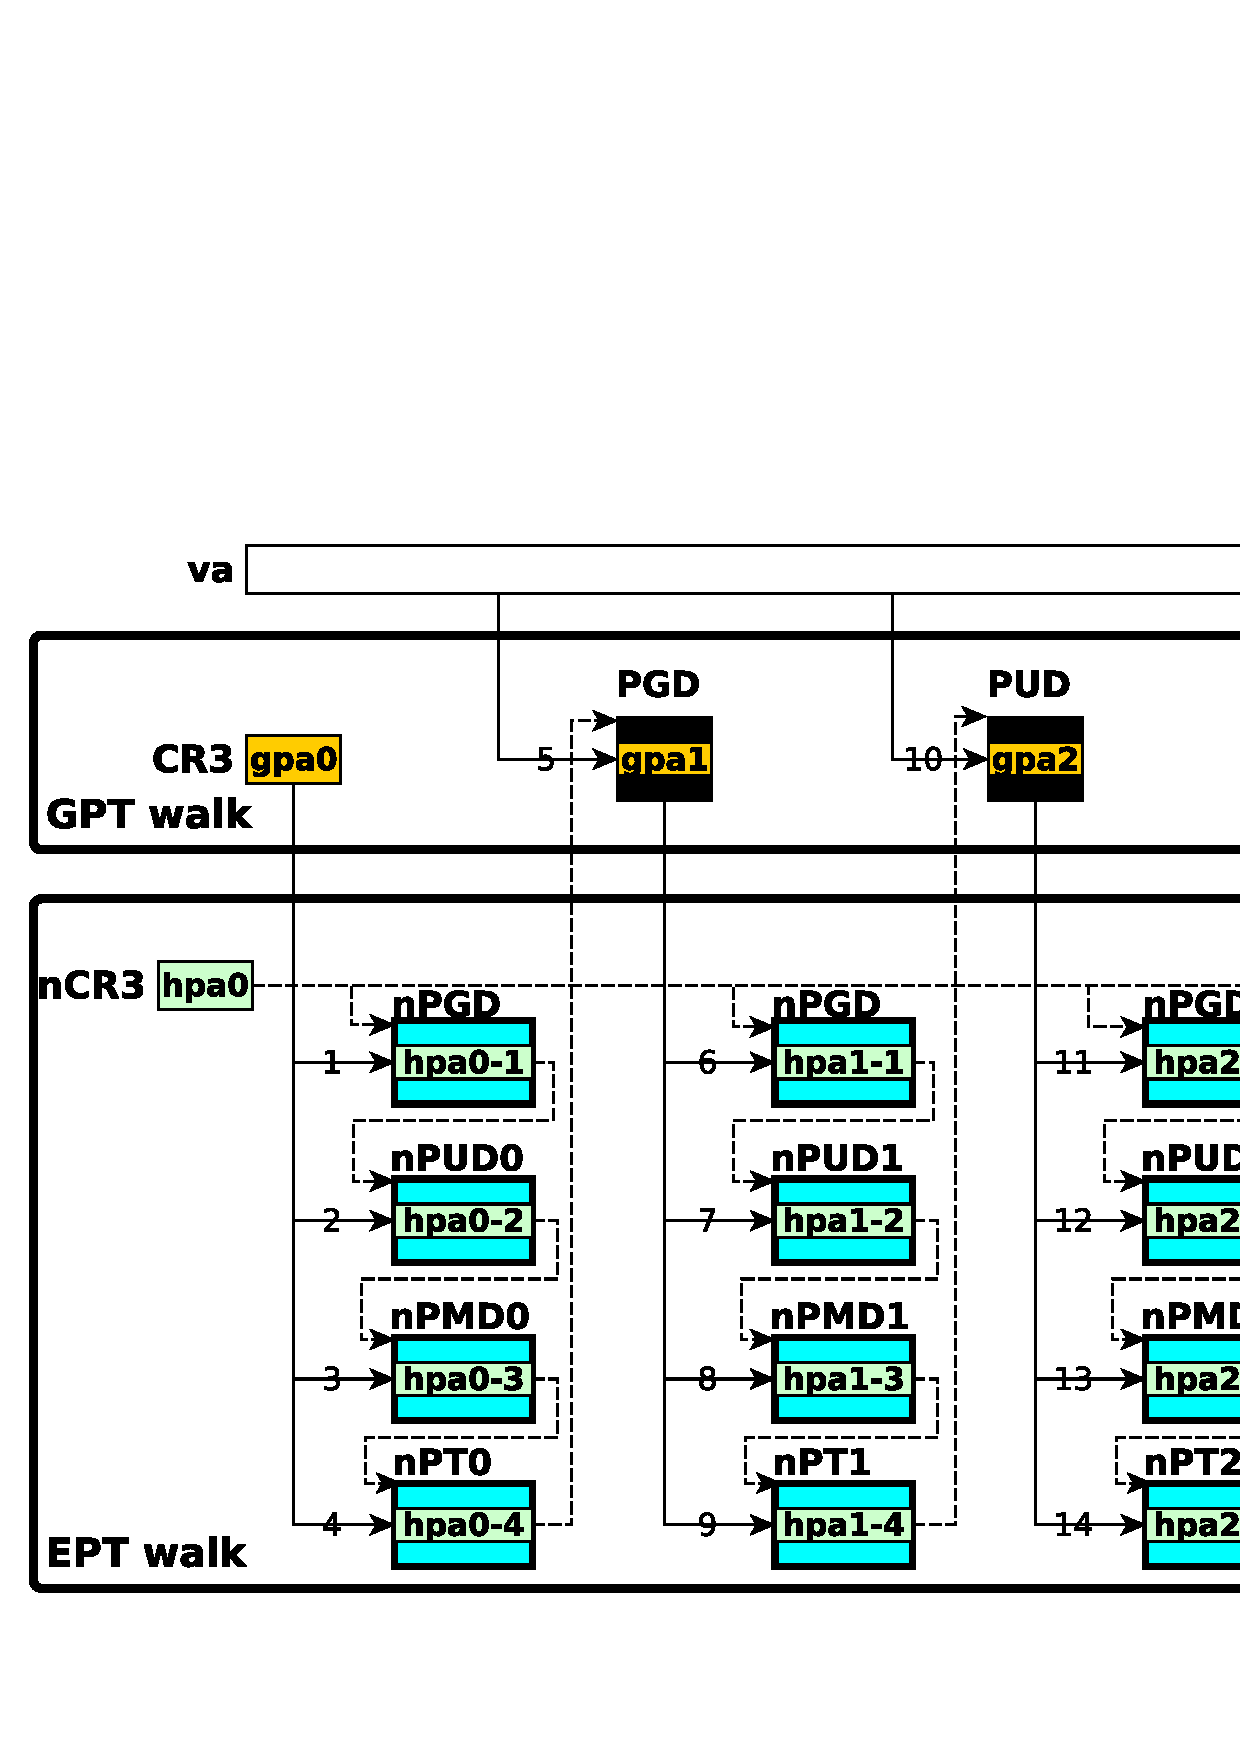
\includegraphics[width=.6\linewidth]{fig/ept.png}				
	% 		\end{subfigure}				
	% 	\end{figure}	
	% \end{overprint}
\end{frame}         
%---------------------------------
\begin{frame}
	\frametitle{OoH for PML}			
	\begin{block}{Two Solutions}
		\begin{itemize}
			\item Shadow PML (SPML): no hardware modification					
			\begin{itemize}
				\item[\ding{50}] Its significant overhead justifies EPML
			\end{itemize}
			\item Extended PML (EPML): modest hardware changes
		\end{itemize}
	\end{block} 
\end{frame}  
%---------------------------------
\begin{frame}
	%\thispagestyle{empty}
	\frametitle{Shadow PML (SPML): Design}
	%\begin{block}{SPML Design}
		\begin{figure}
		\centering
		\fcolorbox{white}{black}{	                					
			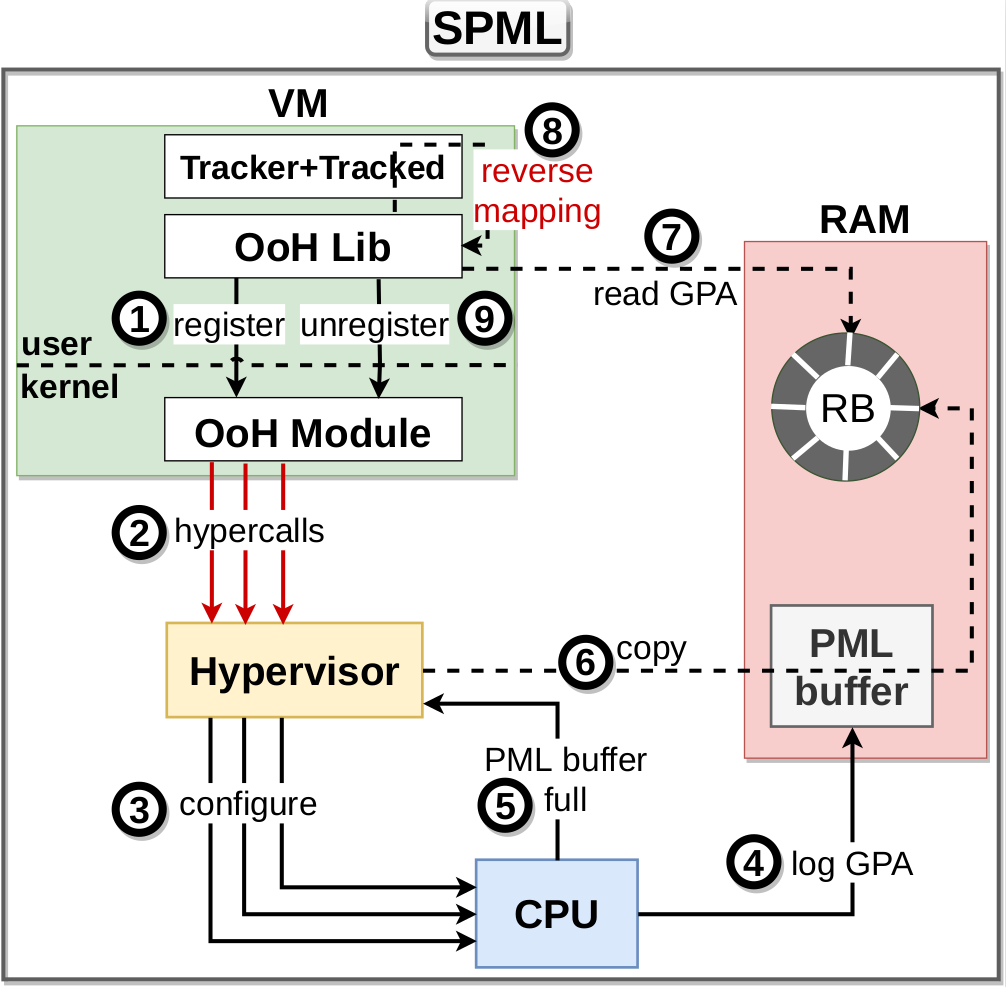
\includegraphics[width=.5\linewidth]{fig/spml.png}
		}				
		\end{figure}
	%\end{block}
\end{frame}
%---------------------------------
\begin{frame}
	\frametitle{Shadow PML (SPML): Limitations}
	\begin{overprint}

		%\onslide<1>
		\begin{itemize}
			\item Costly reverse mapping (\myemph{$\sim$$15.739 \: s$} for 1GB working set)
			\begin{figure}[!h]
				\fcolorbox{white}{white}{	
				\centering 
				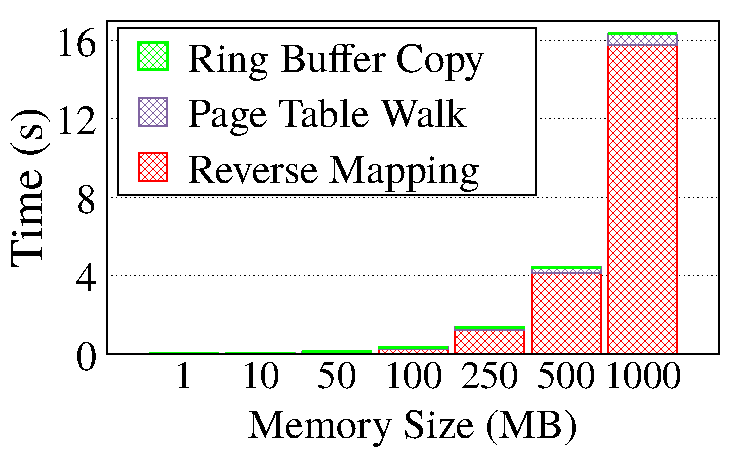
\includegraphics[width=.55\linewidth]{fig/bottleneck}%
				}		
			\end{figure}
			\vspace*{.5cm} 
			\item Costly hypercalls (\myemph{$4.49 \mu s$} for empty hypercall)
		\end{itemize}
~\\
		% %\onslide<2>
		% \begin{itemize}
		% 	\item Costly reverse mapping (\myemph{$\sim$$15.739 \: s$} for 1GB working set)
		% \end{itemize}

	\end{overprint}
\end{frame}
%---------------------------------
\begin{frame}
	\frametitle{Extended PML (EPML): Design}
		
	\begin{overprint}
		\onslide<1>				
		\begin{figure}
		\centering
		\fcolorbox{white}{black}{	                					
			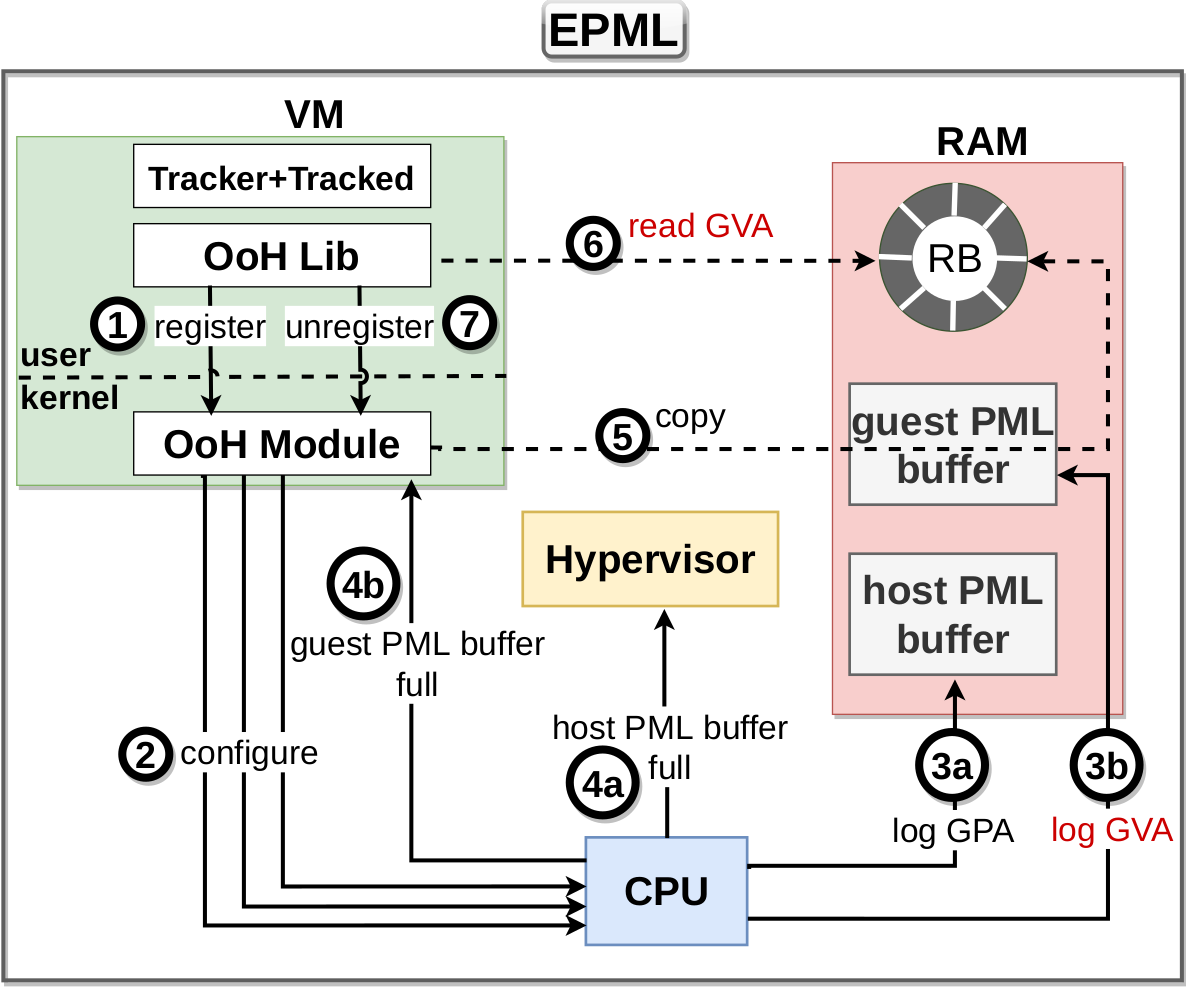
\includegraphics[width=.5\columnwidth]{fig/epml.png}
		}				
		\end{figure} 

	\onslide<2>	
	\begin{figure}
		\centering
		\fcolorbox{white}{black}{	                					
			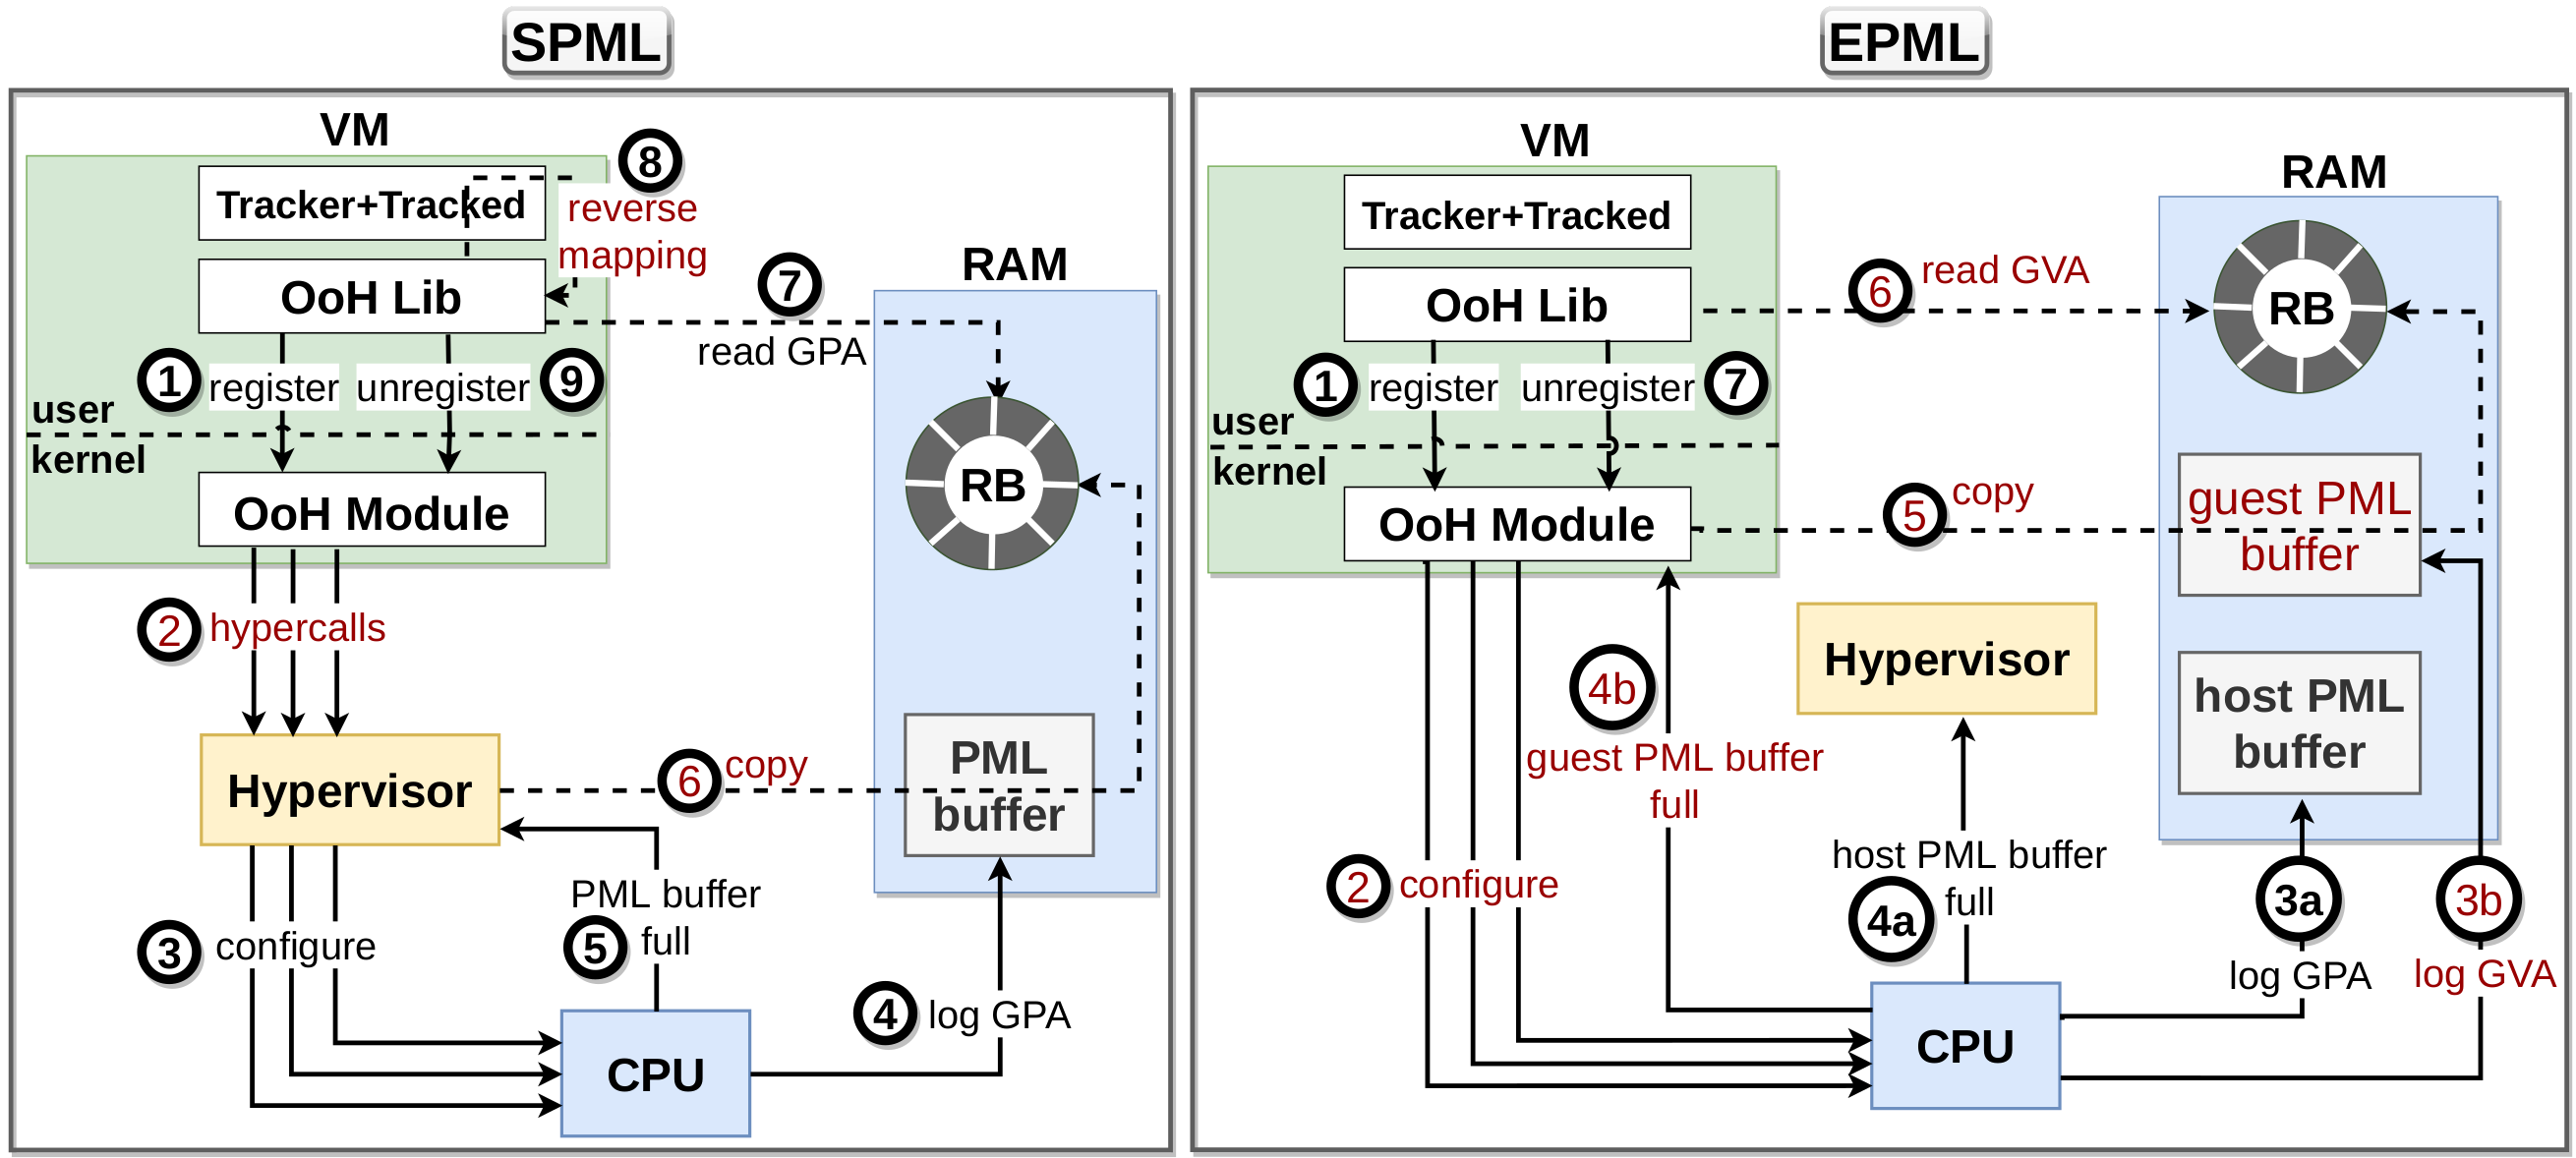
\includegraphics[width=.9\columnwidth]{fig/spml-epml.png}
		}				
		\end{figure}
	\end{overprint}
	
\end{frame}
%---------------------------------
% \begin{frame}
% 	\frametitle{Extended PML (EPML)}			
% 	\begin{itemize}
% 		\item We leverage VMCS shadowing to allow the guest to perform \texttt{vmread} and \texttt{vmwrite} instructions
% 		\item At load time, OoH Module calls the hypervisor to enable and configure VMCS shadowing
% 	\end{itemize}
% \end{frame} 
% %---------------------------------
% \begin{frame}
% 	\frametitle{Extended PML (EPML): Hardware changes}			
% 	\begin{itemize}
% 		\item New VM-Execution Control field in VMCS (called \texttt{Guest PML Address})
% 		\pause
% 		\item PT walk extension
% 		\begin{itemize}
% 			\item GVA logging to the guest-level PML buffer
% 			\item GPA logging to the hypervisor-level PML buffer
% 		\end{itemize} 
% 		\pause
% 		\item Virtual self-IPI\footnote<.(1)->{Inter-Processor Interrupt} raised on guest-level PML buffer is full 
% 	\end{itemize}
% \end{frame}     
%---------------------------------
\begin{frame}
	\frametitle{OoH Security and Isolation}	
	\begin{block}{Vis-à-vis the Hypervisor}		
		\begin{itemize}
			\item Small TCB\footnotemark{} (194LOC) - at least safe as existing hypercalls
			\item Guest does not see nor manipulate host physical memory
			\item Ring buffer allocated from VM's memory
		\end{itemize}
	\end{block}\footnotetext{Trust Code Base}
	\pause
	\begin{block}{Between VMs}		
		\begin{itemize}
			\item Same isolation level 
			\item Ring buffer allocated per VM's address space => no possible inference
			\item Per process ring buffer and restriction to tracker process only
		\end{itemize}		
	\end{block}
\end{frame}     

%%%%%%%%%%%%%%%%%%%%%%%%%%%%%%%%%%%%%%%%%%%%%%%%%%%%%%%%%%%%%%%%%%%%%%%%%%%%%%%%%%%   
\section{Evaluatons}
\subsection{Implementation and Benchmarks}
\subsection{Tracker Evaluation}
\subsection{Tracked Evaluation}
%%%%%%%%%%%%%%%%%%%%%%%%%%%%%%%%%%%%%%%%%%%%%%%%%%%%%%%%%%%%%%%%%%%%%%%%%%%%%%%%%%%
\begin{frame}
	\frametitle{Evaluations: Implementation}
	\begin{itemize}
		\item We implemented EPML's hardware changes in BOCHS				
		\item We used Xen as the hypervisor and Linux as the guest OS
		\item We integrated OoH Lib with: %CRIU and Boehm GC
		\begin{itemize}
			\item[\ding{118}] CRIU: Checkpoint/Restore in User space
			\item[] \begin{itemize}
				\item Integrated in OpenVZ, Docker, etc.
				\item Based on \texttt{/proc} technique
			\end{itemize}
			\item[\ding{118}] Boehm GC: popular C/C++ garbage collector
			\item[] \begin{itemize}
				\item Included in Mozilla, GNU Java Compiler, etc.
				\item Based on \texttt{/proc} technique
			\end{itemize}
		\end{itemize}
	\end{itemize}
\end{frame}
%---------------------------------
\begin{frame}
	\frametitle{Evaluations: Benchmarks}
	\begin{itemize}
		\item Macro-benchmarks: tkrzw applications (key value store) and Phoenix applications (MapReduce)
		\item Three working set sizes (Small, Medium, and Large)
	\end{itemize}
	%\footnotetext[4]{<650MB}\footnotetext[5]{<950MB}\footnotetext[6]{<1.5GB}			
\end{frame}  
%---------------------------------
% \begin{frame}
% 	\frametitle{Evaluations: Questions}	
% 	\begin{block}{$Q1$}
% 		How to accurately evaluate EPML?
% 	\end{block}
% 	\begin{block}{$Q2$}
% 		How do SPML and EPML impact Tracker and Tracked compared to \texttt{/proc} and \texttt{ufd}?	
% 	\end{block}
% 	\begin{block}{$Q3$}
% 		What is the scalability of SPML and EPML?
% 	\end{block}
% \end{frame} 
%---------------------------------
\begin{frame}
	\frametitle{Evaluations: Methodology for EPML}
	Approach
	\begin{itemize}
		\item Build a formula $f$
		\item Show the accuracy of $f$ on other techniques that are measurable
	\end{itemize}
\end{frame}
%---------------------------------
\begin{frame}
	\frametitle{Evaluations: Methodology for EPML}
	%Can be applied to each tracking technique			
	\begin{block}{Impact on Tracker}
		Execution time of Tracker when implementing technique $x$:\\
		$E(C_{tker}) = E(C_{x}) + E(C_{p}) + I(C_{x},C_{p})$
		~\\
		$x$: \textit{\texttt{/proc}, SPML, EPML} -
		$C_{x}$: \textit{enable\_PML, ring buffer copy, etc.}
	\end{block} 
~\\~\\
	\begin{block}{Impact on Tracked}
		Time of Tracked when monitored by a Tracker using technique $x$:\\
		$E(C_{tked\_tker}) = E(C_{tked}) + E(C_{tker}) + I(C_{x},C_{tked})$
		~\\
		$I(C_{x},C_{tked})$: \textit{page faults, vmexits, etc.}
	\end{block}
\end{frame}                                                                              
%---------------------------------
% \begin{frame}
% 	\frametitle{Evaluations}
% 	\begin{block}{Formulas: Impact on Tracker}
% 		Formula 1 pplied to each technique:
% 		\begin{equation}\scriptsize
% 			\begin{split}
% 				E(C_{/proc}) = & \; E(C_{echo \; 4 \; > \; /proc/PID/clear\_refs}) \\
% 							& + E(C_{page \; table \; walk \; in \; userspace}) \\
% 				E(C_{UFD}) = & \; E(C_{ioctl \; write\_protect}) \\
% 							& + E(C_{ioctl \; register}) \\
% 							& + E(C_{ioctl \; write\_unprotect}) \\
% 				E(C_{SPML}) = & \; E(C_{ring \; buffer \; copy}) \\
% 							& + E(C_{reverse \; mapping}) \\
% 							& + E(C_{enable/disable \; PML}) \\
% 				E(C_{EPML}) = & \; E(C_{ring \; buffer \; copy}) \\
% 							& + E(C_{enable/disable \; PML})
% 			\end{split}
% 			\label{eq:formula-detailed}
% 		\end{equation}								
% 	\end{block}
% \end{frame}
%---------------------------------
% \begin{frame}
% 	\frametitle{Evaluations}			
% 	\begin{block}{Formulas: Impact on Tracked}
% 		Generic formula:
% 		\begin{itemize}
% 			\item Execution time of Tracked when monitored by a Tracker using technique $x$:
% 			\begin{equation}
% 				\small
% 				\label{eq:formula-tracked}
% 				E(C_{tked\_tker}) = E(C_{tked}) + E(C_{tker}) + I(C_{x},C_{tked})
% 			\end{equation}
% 			$I(C_{x},C_{tked})$: page faults, vmexits, etc.
% 			$E(C_{tker}) + I(C_{x},C_{tked})$: overhead of $x$ on Tracked 
% 		\end{itemize}
% 	\end{block} 
% \end{frame}        
% %---------------------------------
% \begin{frame}
% 	\frametitle{Evaluations}
% 	\begin{block}{Formulas: Impact on Tracked}
% 		Formula 3 applied to each technique:
% 		\begin{equation}\scriptsize
% 			\begin{split}
% 				I(C_{/proc},C_{tked}) = & \; E(C_{PFH \; in \; kernelspace})\\
% 										& + E(C_{context \; switch})\\
% 				I(C_{UFD},C_{tked}) = & \; E(C_{PFH \; in \; userspace})\\
% 									& + E(C_{context \; switch}) \\
% 				I(C_{SPML},C_{tked}) = & \; E(C_{vmexits}) \\
% 									& + N \times E(C_{vmread/vmwrite})\\
% 				I(C_{EPML},C_{tked}) = & \; N \times E(C_{vmread/vmwrite})	
% 			\end{split}
% 			\label{eq:formula-impact-detailed}
% 		\end{equation}		
% 		In $I(C_{EPML},C_{tked})$, N\footnotemark{} is the same as for SPML (validated by running SPML and EPML under BOCHS).
% 	\end{block}\footnotetext{Number of context switches}
% \end{frame}   
%---------------------------------
\begin{frame}
	\frametitle{Evaluations: Formulas Validation}
	\begin{table}[h]
		\centering \scriptsize
		\begin{subtable}[b]{.45\textwidth}
			\centering 
			\begin{tabular}{l l}
				\toprule
				\hline
				Metric & Time (ms) \\
				\hline
				\textcolor{americanrose}{\textbf{$E(C_{tker})$}} & \\
				\textcolor{americanrose}{\textbf{measured}} & \multirow{-2}{*}{\textcolor{americanrose}{\textbf{5503.79}}}\\
				\textcolor{airforceblue}{\textbf{$E(C_{tked\_tker})$}} & \\
				\textcolor{airforceblue}{\textbf{measured}} & \multirow{-2}{*}{\textcolor{airforceblue}{\textbf{135255.35}}}\\
				\midrule
				$E(C_{p})$ & 251.35\\
				$E(C_{copy\_rb})$ & 0.49\\
				$E(C_{disable \; pml})$ & 2.06\\
				$E(C_{rev. \; mapping})$ & 5419 \\
				\textcolor{americanrose}{\textbf{$E(C_{tker})$}}  &\\
				\textcolor{americanrose}{\textbf{estimated}} &  \multirow{-2}{*}{\textcolor{americanrose}{\textbf{5672.9}}}\\
				\midrule
				$E(C_{vmexits})$ & 18000\\
				$N$ & 39\\
				$E(C_{vmread,vmwrite})$ & $1.73 \times 10^{-3}$\\
				\textcolor{airforceblue}{\textbf{$E(C_{tked\_tker})$}}  & \\
				\textcolor{airforceblue}{\textbf{estimated}} & \multirow{-2}{*}{\textcolor{airforceblue}{\textbf{136919.85}}}\\
				\bottomrule
			\end{tabular}
			\subcaption{SPML}
			\label{tab:criu-spml-formula}
		\end{subtable}
		\hfill
		\begin{subtable}[b]{.45\textwidth}
			\centering 
			\begin{tabular}{l l}
				\toprule
				\hline
				Metric & Time (ms) \\
				\hline
				\textcolor{americanrose}{\textbf{$E(C_{tker})$}} & \\
				\textcolor{americanrose}{\textbf{measured}} & \multirow{-2}{*}{\textcolor{americanrose}{\textbf{1097.99}}}\\
				\textcolor{airforceblue}{\textbf{$E(C_{tked\_tker})$}} & \\
				\textcolor{airforceblue}{\textbf{measured}} & \multirow{-2}{*}{\textcolor{airforceblue}{\textbf{115283.98}}}\\
				\midrule
				$E(C_{p})$ & 251.35\\
				$E(C_{clear\_refs})$ & 1.409\\
				$E(C_{PT walk})$ & 0.89\\
				\textcolor{americanrose}{\textbf{$E(C_{tker})$}}  & \\
				\textcolor{americanrose}{\textbf{estimated}} & \multirow{-2}{*}{\textcolor{americanrose}{\textbf{1116.09}}}\\
				\midrule
				$E(C_{PFH user})$ & 0.27\\
				\textcolor{airforceblue}{\textbf{$E(C_{tked\_tker})$}}  &\\
				\textcolor{airforceblue}{\textbf{estimated}} &  \multirow{-2}{*}{\textcolor{airforceblue}{\textbf{114418.58}}}\\
				\bottomrule
			\end{tabular}
			\subcaption{\texttt{/proc}}
			\label{tab:criu-proc-formula}
		\end{subtable}
		\vspace{.3cm}
		\caption{An accuracy of 96.34\% and 99\% respectively}
		\vspace{.3cm}
	\end{table}
\end{frame}  
%---------------------------------
\begin{frame}
	\frametitle{Evaluations: Formulas Validation}
	\begin{center}
		SPML accuracy: \myemph{96.34\%}\\
		~\\
		\texttt{/proc} accuracy: \myemph{99\%}		
	\end{center}
\end{frame}                 
%---------------------------------
\begin{frame}
	\frametitle{Evaluations: Tracker Results}
	Boehm \hspace*{3cm} CRIU
	\begin{figure}[!h]
		\centering 
		\begin{subfigure}[m]{.32\linewidth}
			\centering
			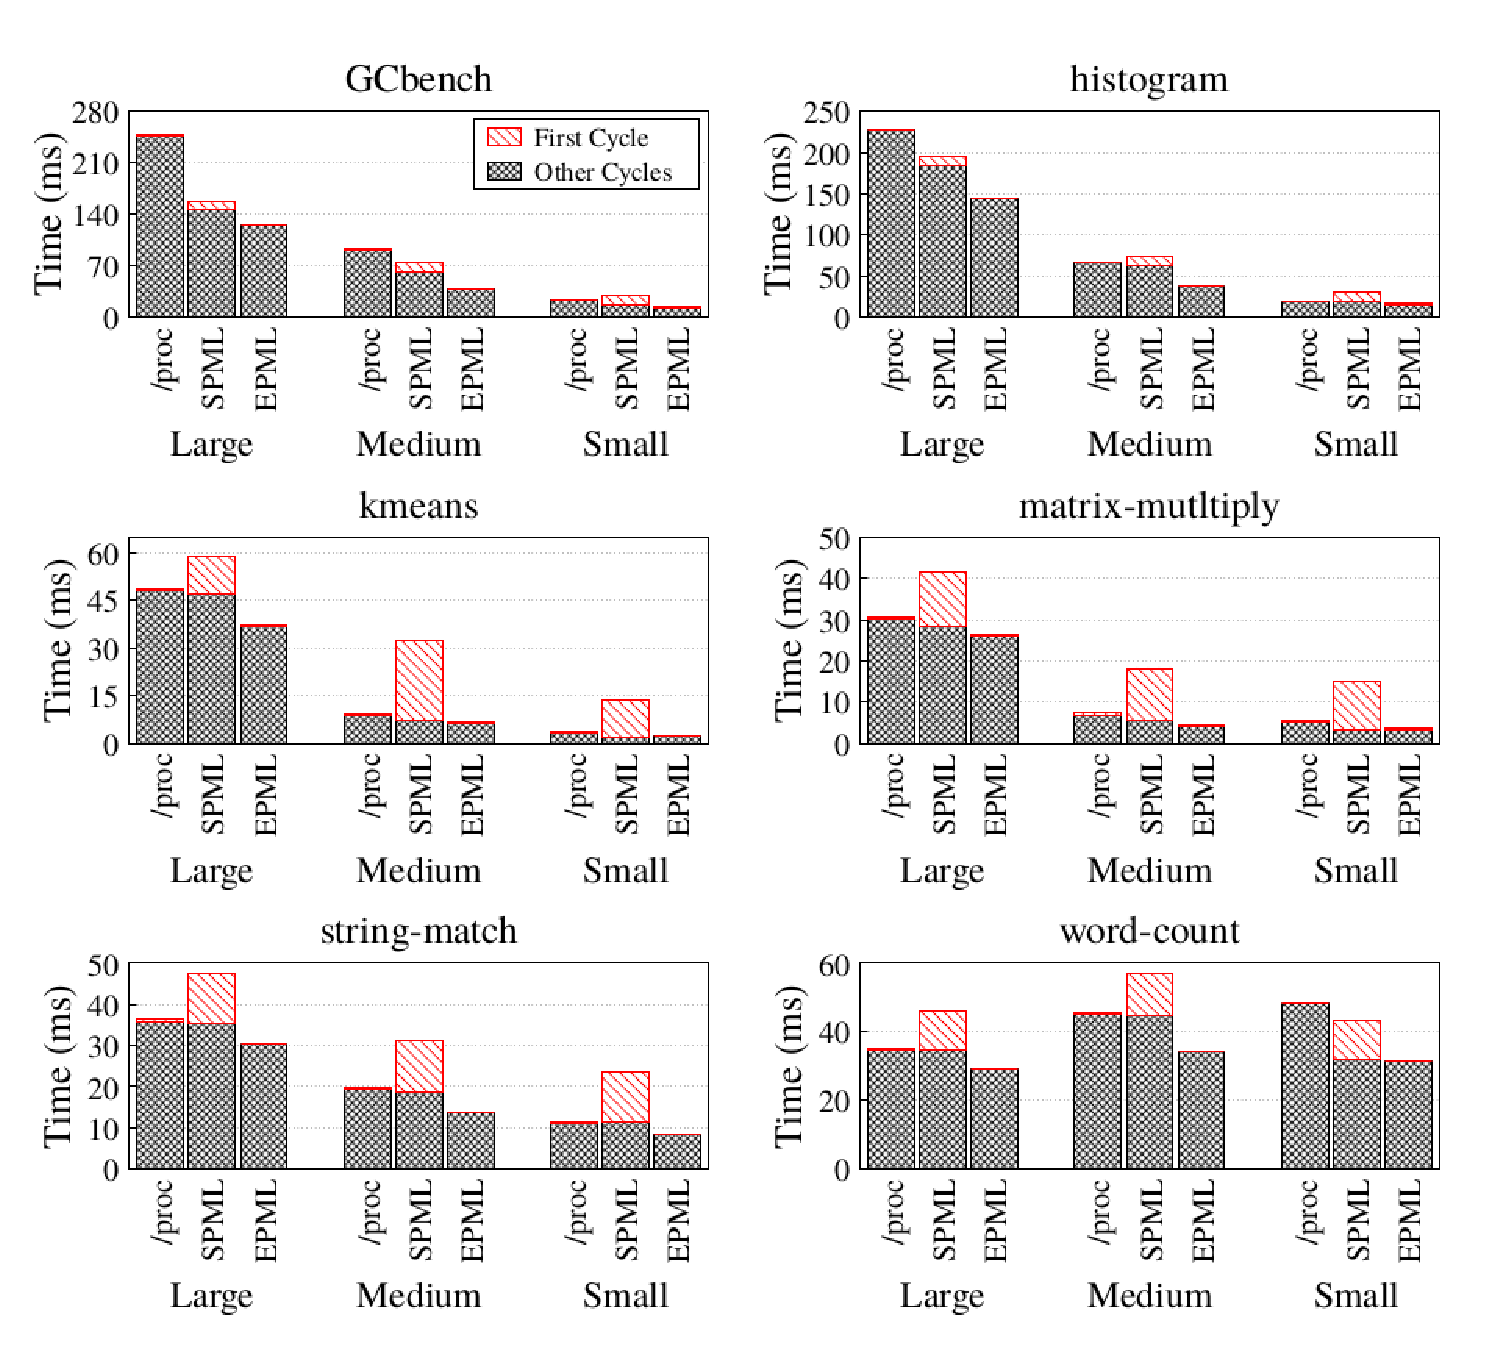
\includegraphics[width=\linewidth]{fig/boehm-results-tracker}			
		\end{subfigure}	
		\hfill
		\begin{subfigure}[m]{.32\linewidth}
			\centering
			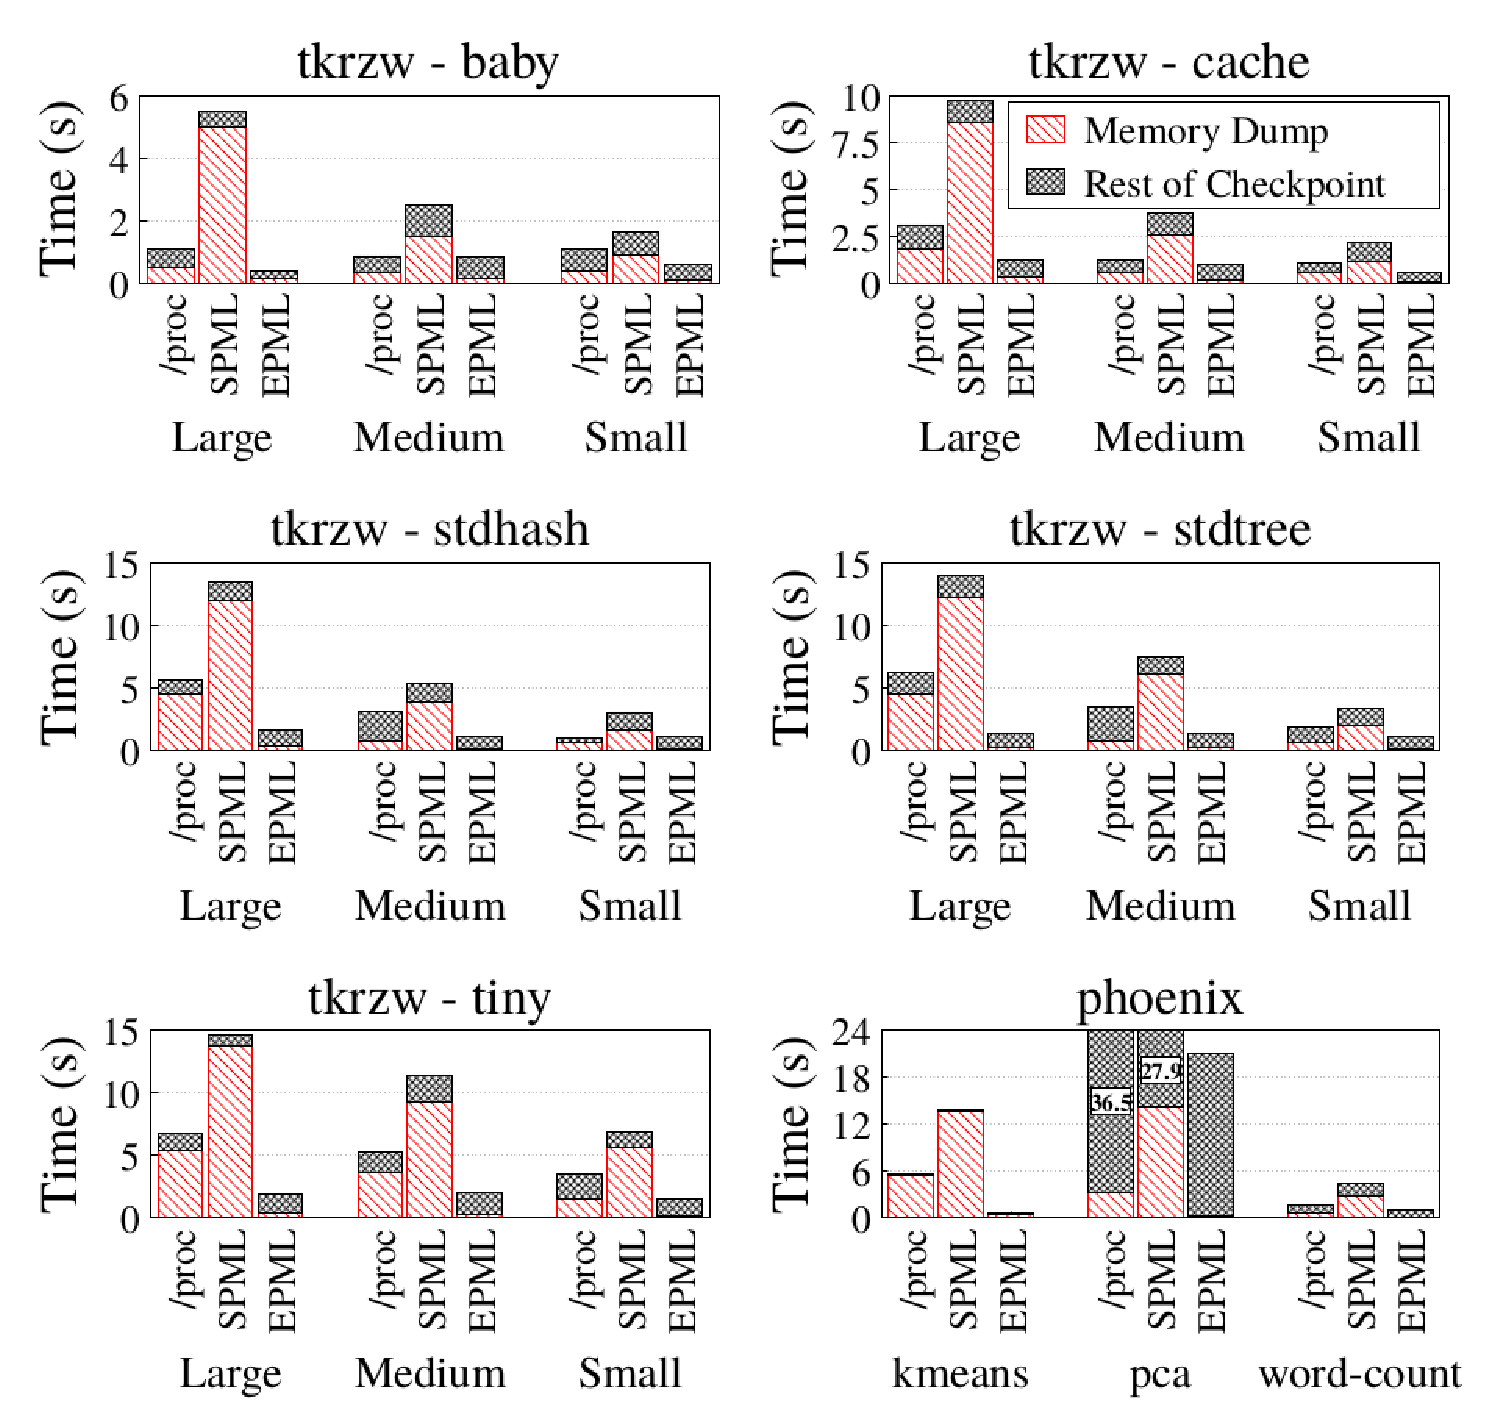
\includegraphics[width=\linewidth]{fig/criu-results-tracker}			
		\end{subfigure}		
		\hfill
		\begin{subfigure}[m]{.34\linewidth}
			%\centering
			SPML vs. \texttt{/proc}: \myemph{5$\times$} and \myemph{3$\times$} slowdown resp. on CRIU and Boehm	\\	
			~\\		
			\noindent EPML: (\textcolor{blue}{\bf On CRIU:}) \myemph{4$\times$} and \myemph{13$\times$} speedup compared to \texttt{/proc} and SPML resp.\\
			\noindent (\textcolor{blue}{\bf On Boehm:}) \myemph{2$\times$} and \myemph{6$\times$} speedup compared to \texttt{/proc} and SPML resp.
		\end{subfigure}	
	\end{figure}											
\end{frame}
%---------------------------------
% \begin{frame}
% 	\frametitle{Evaluations: Results Summary}
% 	\begin{block}{Impact on Tracker}
% 		\begin{itemize}
% 			\item<1-> SPML compared to default (\texttt{/proc}): 
% 			\begin{itemize}
% 				\item On CRIU: \myemph{5$\times$} slowdown
% 				\item On Boehm GC: \myemph{3$\times$} slowdown
% 			\end{itemize}
			
% 			\item<2-> EPML: 
% 			\begin{itemize}
% 				\item On CRIU: \myemph{4$\times$} and \myemph{13$\times$} speedup compared to \texttt{/proc} and SPML resp.
% 				\item On Boehm GC: \myemph{2$\times$} and \myemph{6$\times$} speedup compared to \texttt{/proc} and SPML resp.
% 			\end{itemize}
% 		\end{itemize}																				
% 	\end{block}
% \end{frame}  
%---------------------------------
\begin{frame}
	\frametitle{Evaluations: Tracked Results}
	\centering Boehm
	\begin{figure}[!htp]
		\centering
		\begin{subfigure}{\linewidth}
			\centering
			\fcolorbox{white}{white}{
				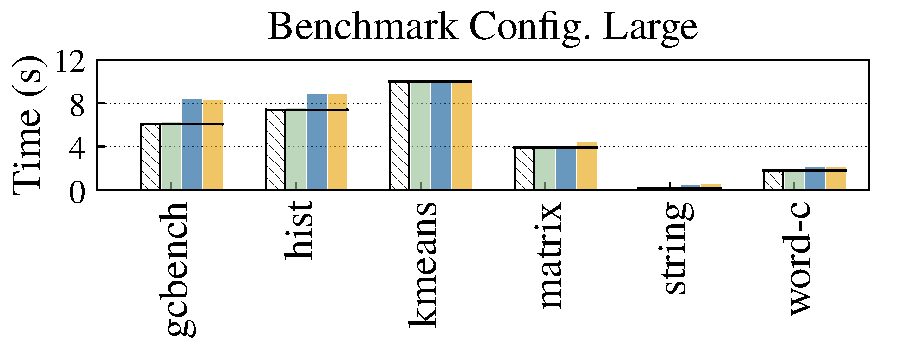
\includegraphics[width=.3\linewidth]{fig/tracked_large_boehm}
				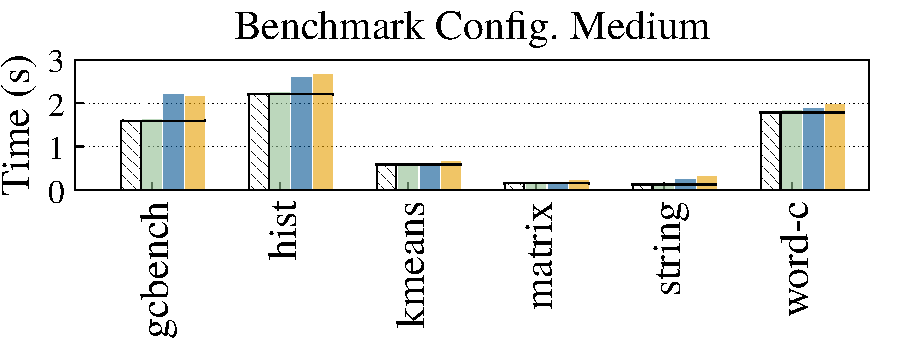
\includegraphics[width=.3\linewidth]{fig/tracked_medium_boehm}
				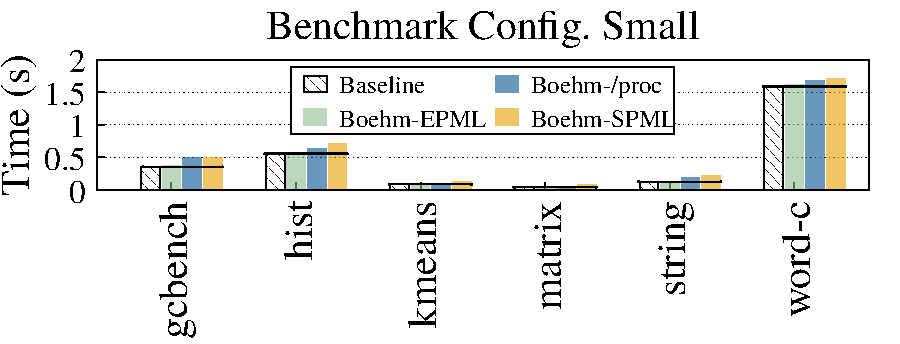
\includegraphics[width=.3\linewidth]{fig/tracked_small_boehm}
			}			
		\end{subfigure}
	\end{figure}
	\centering CRIU
	\begin{figure}[!htp]
		\begin{subfigure}{\linewidth}
			\centering
			\fcolorbox{white}{white}{
			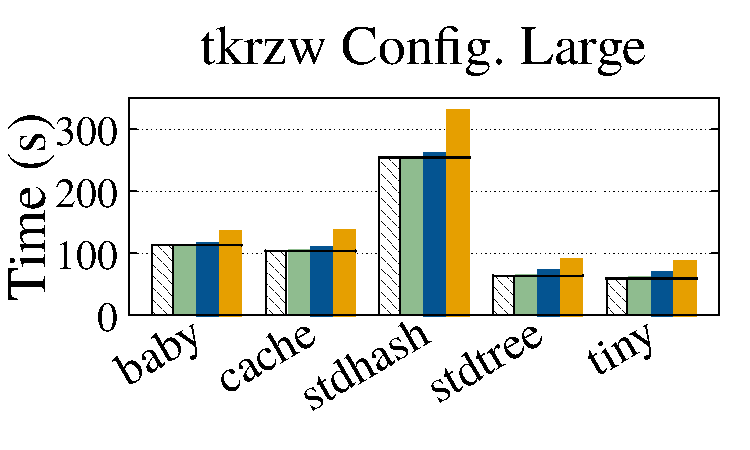
\includegraphics[width=.3\linewidth]{fig/tracked_large}
			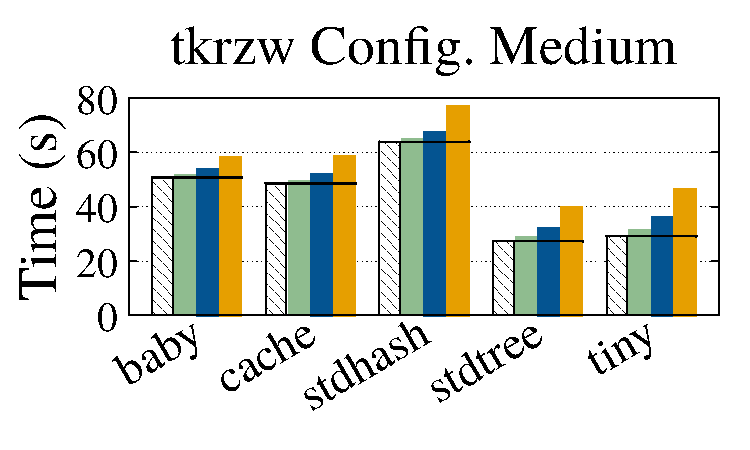
\includegraphics[width=.3\linewidth]{fig/tracked_medium}
			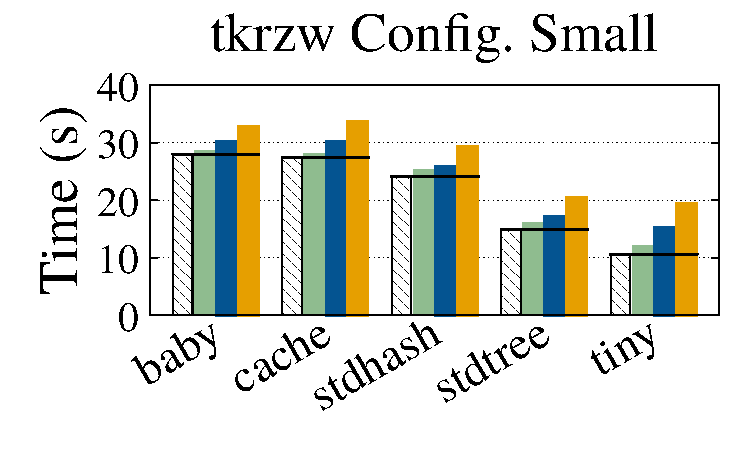
\includegraphics[width=.3\linewidth]{fig/tracked_small}
			}			
		\end{subfigure}
		% \caption{\small Impact of Boehm GC.}
		% \label{fig:boehm-results-tracked}
	\end{figure}
\end{frame}         
%---------------------------------
\begin{frame}
	\frametitle{Evaluations: Tracked Results}
	\begin{block}{Impact on Tracked}
		\begin{itemize}	
			\item \textcolor{blue}{\bf \texttt{/proc}}: 
			\begin{itemize}
				\item Up to \myemph{102\%} overhead on Phoenix-\texttt{pca} with CRIU
				\item Up to \myemph{232\%} overhead on Phoenix \texttt{string-match} with Boehm
			\end{itemize}

			\item \textcolor{blue}{\bf SPML}: 
			\begin{itemize}
				\item Up to \myemph{114\%} overhead on Phoenix-\texttt{pca} with CRIU
				\item Up to \myemph{273\%} overhead on Phoenix \texttt{string-match} with Boehm
			\end{itemize}
			
			\item \textcolor{blue}{\bf EPML}: 
			\begin{itemize}
				\item Only \myemph{7\%} with CRIU
				\item Only \myemph{24\%} with Boehm
				\item ==> \myemph{16$\times$} improvement
			\end{itemize}
																			
		\end{itemize}
	\end{block}
\end{frame}              

\setbeamertemplate{headline}{}
%\setbeamertemplate{footline}{\textit{Stella Bitchebe (bitchebe@i3s.unice.fr) \& Alain Tchana (alain.tchana@ens-lyon.fr)} 
\includegraphics[width=.1\linewidth]{images/logobottom.png}  \hspace{-6cm}\vspace{3cm}}
%%%%%%%%%%%%%%%%%%%%%%%%%%%%%%%%%%%%%%%%%%%%%%%%%%%%%%%%%%%%%%%%%%%%%%%%%%%%%%%%%%%   
\section{Conclusion}
%%%%%%%%%%%%%%%%%%%%%%%%%%%%%%%%%%%%%%%%%%%%%%%%%%%%%%%%%%%%%%%%%%%%%%%%%%%%%%%%%%%
\begin{frame}
\thispagestyle{empty}
\frametitle{Conclusion} 
	Dirty Page Tracking
	\begin{itemize}
		\item For wss estimation, live migration, checkpointing, GC, ...
		\item Induce high overhead on applications
	\end{itemize}
	\vspace*{.5cm}
	\pause
	OoH for Intel PML (\textcolor{blue}{\bf \url{https://github.com/bstellaceleste/OoH}})
	\begin{itemize}
		\item For improving process/container checkpointing, concurrent GCs
		\item \myemph{4$\times$} speedup on Tracker - \myemph{16$\times$} improvement on Tracked
	\end{itemize}
	\vspace*{.5cm}
	\pause
	Take Away
	\begin{itemize}
		\item Existing sofware-based tools can be improved using hardware virtualization features
		\item Think of OoH from the conception/design of hardware virtualization features
		%When thinking hardware virtualization features, we must think how they can also be used by processes from inside VMs, this may need few efforts
	\end{itemize}					
\end{frame}                       
%---------------------------------
% \begin{frame}
% 	\thispagestyle{empty}
% 	\frametitle{Conclusion} 
% 	\begin{block}{Current Work: OoH for SPP}
% 		\begin{itemize}
% 			\item For improving secure heap memory allocators that run from inside VMs
% 			\item Induce high overhead on applications
% 		\end{itemize}
% 	\end{block}						
% \end{frame}  
\frame[plain]{
\includegraphics[page=1,width=\textwidth]{title.pdf}}

\end{document}
